\documentclass[a4paper, 11pt]{article}
\usepackage[mode=buildnew]{standalone}
\usepackage[utf8]{inputenc}
\usepackage[margin=2.5cm]{geometry}
\usepackage{graphicx}
\usepackage{siunitx}
\usepackage{float}
\usepackage{microtype}
\usepackage{subcaption}
\usepackage{caption}
\captionsetup{font=small}
\captionsetup[subfigure]{width=0.9\linewidth}
\captionsetup[figure]{width=0.8\linewidth}
\captionsetup[table]{width=0.8\linewidth}
\usepackage{hyperref}
\usepackage{amsmath}
\usepackage[nameinlink,noabbrev,capitalise]{cleveref}
\usepackage{booktabs}
\usepackage{tabulary}
\usepackage{appendix}
\usepackage{tikz}

\usepackage{import}

\usepackage{fancyhdr}
\setlength{\headheight}{14pt}
\fancyhead[L]{Integrated Design Project}
\fancyhead[R]{}
\pagestyle{fancy}

\title{IDP Report}
\author{L221}
\date{February 2021}


\usepackage{titling}
\makeatletter
\renewcommand{\maketitle}{
\begin{titlingpage}
\begin{center}
    \vspace*{4cm}
    {\Huge\bfseries\@title}\par
    \vspace*{2cm}
    \Large
    \@author\par\bigskip
    Trinity College\par
    \vspace*{2cm}
    \@date
\end{center}
\end{titlingpage}
}
\makeatother


%%--------------------------------------------------------------------------
%% Code Highlighting
%%--------------------------------------------------------------------------

\usepackage{xcolor}
\usepackage{listings}
\definecolor{pyorange}{RGB}{255,119,0}
\definecolor{pyblue}{RGB}{0,0,255}
\definecolor{pypurple}{RGB}{144,0,144}
\definecolor{pyred}{RGB}{221,0,0}
\definecolor{pygreen}{RGB}{0,170,0}
\definecolor{pyblack}{RGB}{0,0,0}
\lstdefinestyle{pystyle}{
    commentstyle = \color{pygreen},
    keywordstyle = \color{pyblue},
    stringstyle = \color{pyorange},
    basicstyle = \small\color{pyblack}\ttfamily,
    breaklines = true, %automatic line breaking of long lines      
    numbers = left,
    numberstyle=\tiny,
    showstringspaces = false,
    stepnumber = 2,
	xleftmargin=17pt,
	captionpos=b
}
\lstset{style=pystyle,language=Python}


%%--------------------------------------------------------------------------
%% References
%%--------------------------------------------------------------------------

\usepackage[style=nature]{biblatex}
% \bibliography{bibliography.bib}


% - Mechanical
% - Sketches of the concepts you have considered (which may be photocopied/scanned from your lab book). Evaluation charts of these concepts together with a brief discussion of the advantages and disadvantages of each
% - *Robot Concept and diagram.* This could be hand-drawn diagrams, CAD models or any format which conveys the approach and concept

% - Electrical
% - *Electronics/Sensing.* This should include a list of sensors/circuits required, any circuit diagrams/block diagrams which may have already been developed. Discussion as to if/why some processing will be performed in electronics opposed to software (e.g. obtaining digital outputs from analogue signals)
% - Overall System Level Diagram. Detailing how the electronics, hardware and software interacts
% - Integration between hardware electronics and software

% - What is the most risky/challenging aspect of the project?
% - Gantt Chart (resource/time allocation)
% - Approach for solving the problem

% - Software
% - *Software.* Exploration and navigation algorithms. Interface to electronics, discussion of choice of algorithms, any failure detection/recovery which will be implemented.




\begin{document}

\maketitle


\section{Project Management}

\subsection{Team organisation}

The team is divided into 3 sub-teams, each holding responsibility for the progress of each aspect of the project; we have a mechanical, electrical and software sub-team. The teams are split with Youjing and Care (Raksina) in the mechanical team, Eleanor and Karl in the electrical team and Weixuan, Jason and Ghifari in the software team. We also have Ghifari as the team leader, responsible for project management.


Although we have these 3 distinct teams, an interdisciplinary approach is taken. All 3 teams are in constant communication to ensure that a holistic view is taken for any decisions that need to be made. This is true for anything from the Overall Robot Strategy to the chassis design.

\subsection{Approach}

Our approach to tackling this problem is to use the Agile methodology. First, we collectively agreed on a Minimum Viable Product (MVP) that we aim to create as soon as possible. Once this is created, we go through week-long iterations of optimising and overcoming any problems before a review of progress every Saturday. In this way we have a clear direction in terms of what we need to achieve and for when.

The current MVP comprises of a few details from each team. From the mechanical team, it is a simple model of the chassis in Webots with rough, initial dimensions; from the electrical team, it is to create the lookup tables for the sensors we will be using (long IR and ultrasonic sensors) and from the software team, it is a robot with simple motion controls that can detect a block and go towards it.

\subsection{Gantt Chart}

\begin{figure}[H]
    \centering
    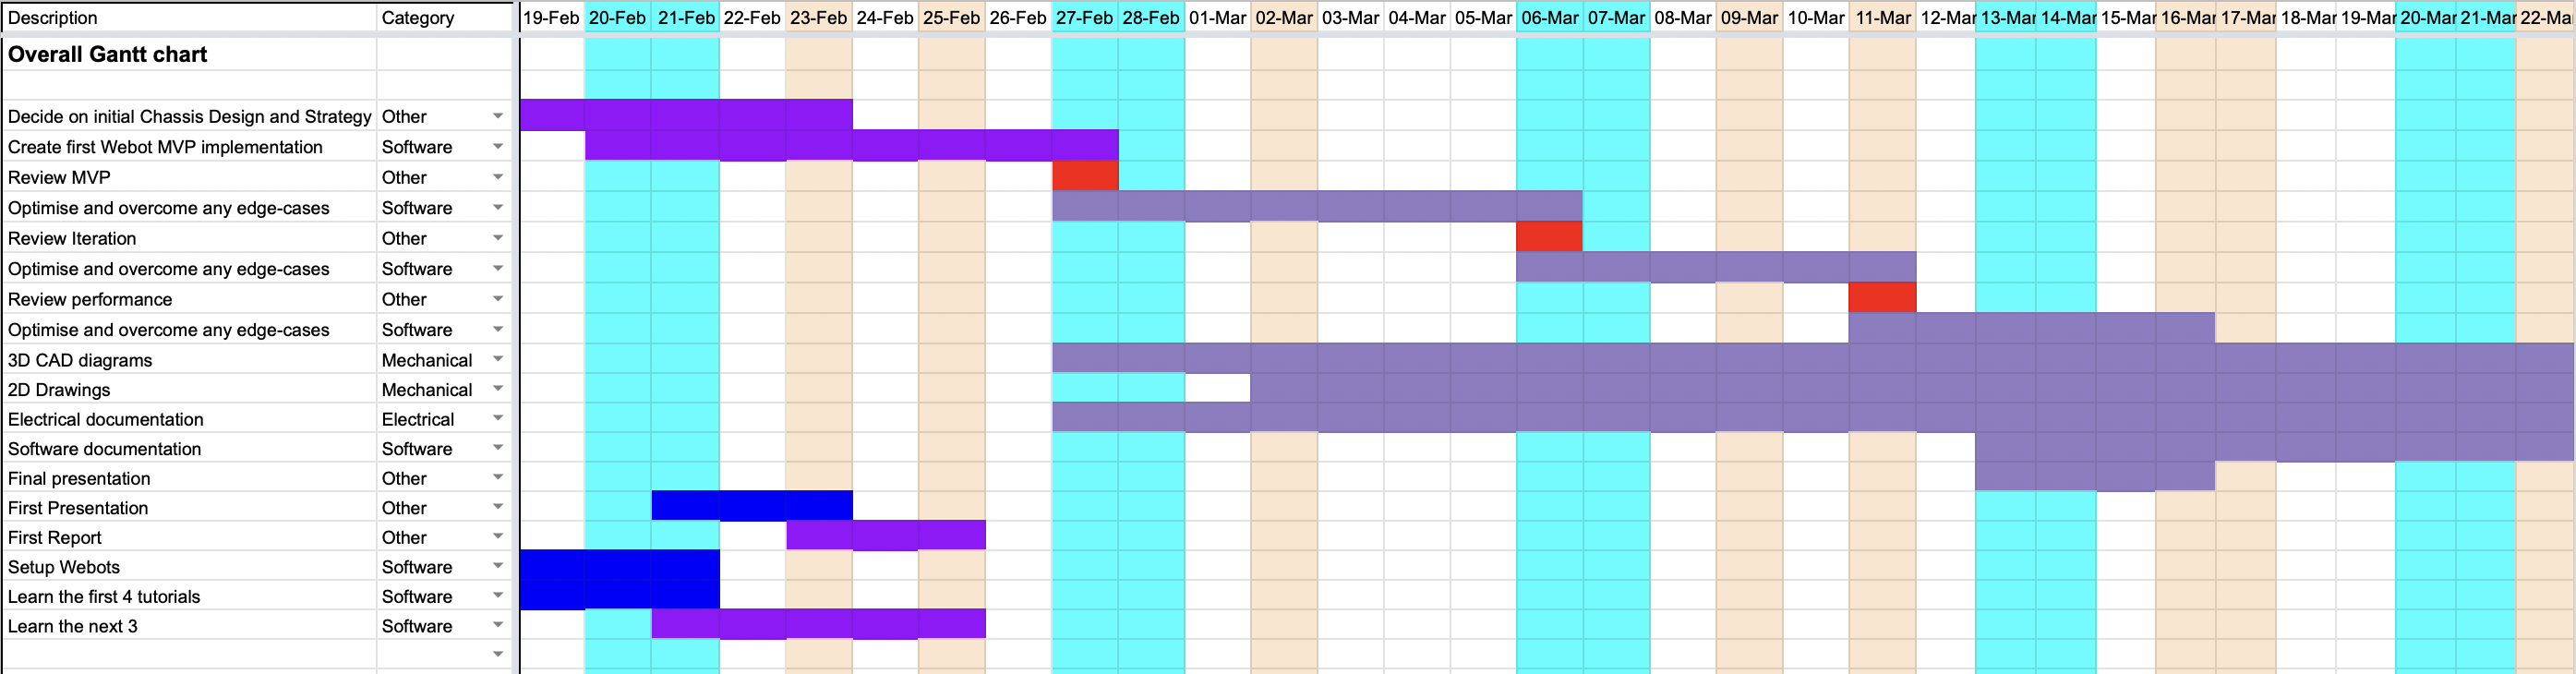
\includegraphics[width=\textwidth]{GanttChart}
    \caption{Overall team Gantt Chart}
    \label{fig:gantt_chart}
\end{figure}


\cref{fig:gantt_chart} shows our timeline for the project. We are currently in progress to meet the MVP deadline of this Saturday, which is currently the most critical path. Saturday's meeting will enable important tasks to start such as the 3D CAD drawings and electrical documentation.


\section{Mechanical}
\subsection{Initial Designs}

\begin{figure}[H]
    \centering
    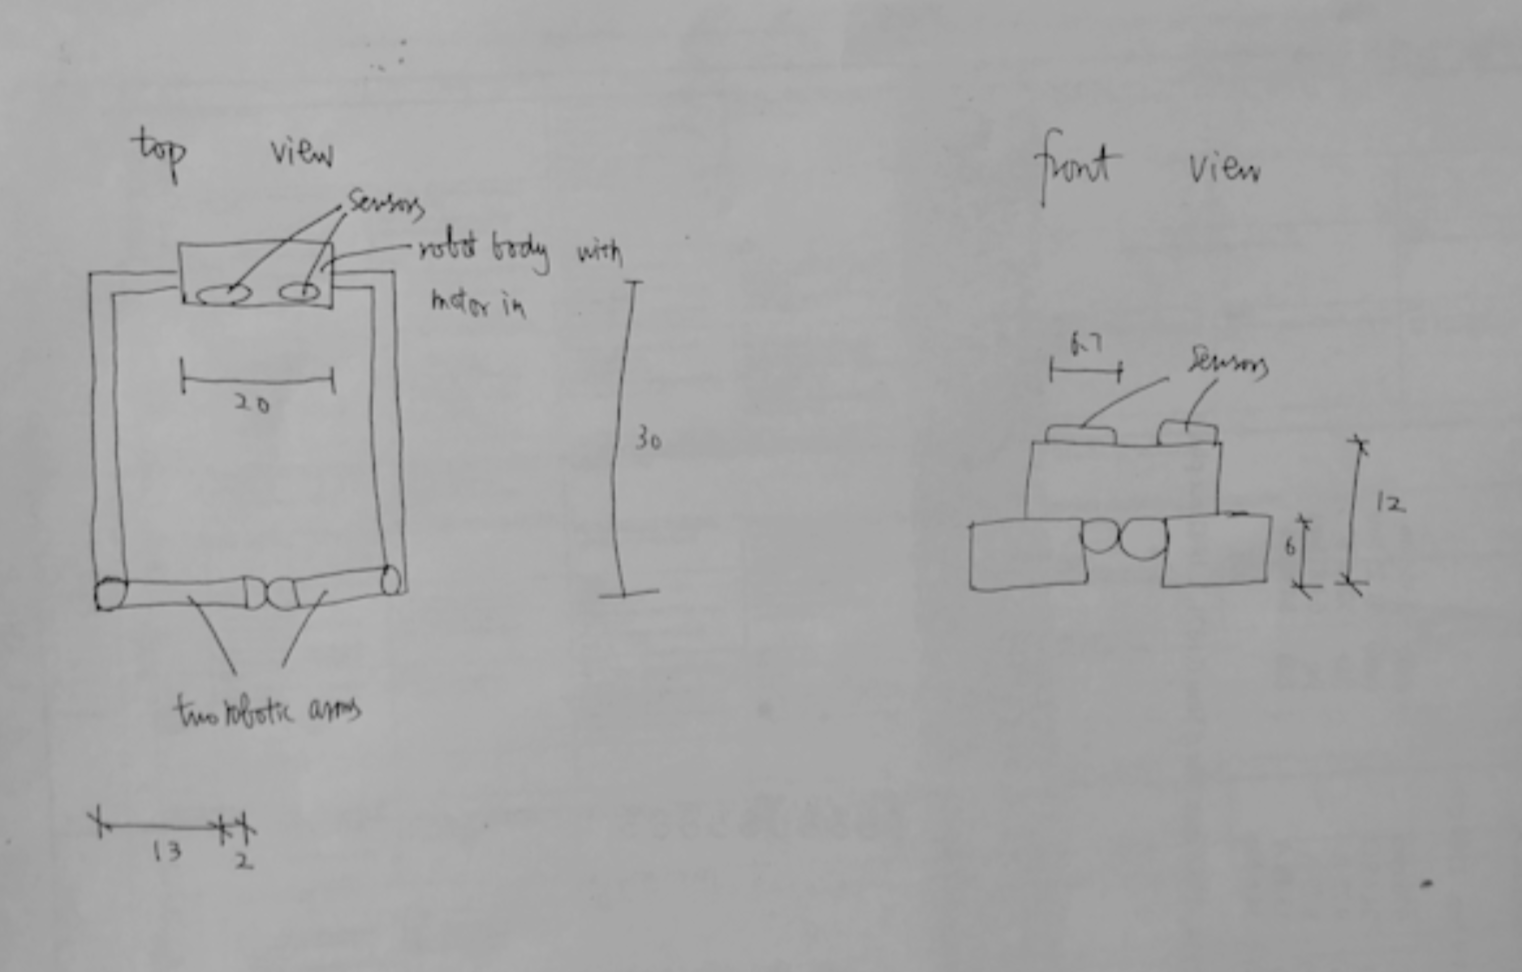
\includegraphics[width=8cm]{Design1}
    \caption{The First Design}
\end{figure}


The pros of the designs are that it is symmetric so it will be easier for sensor construction and placement. It is also a relatively simple design to recreate. However, this design suffers from the shortcomings that the sensor is at the back of the robot, which makes it difficult for the blocks to be accurately detected. The square shape also makes it difficult to rotate.


\begin{figure}[H]
    \centering
    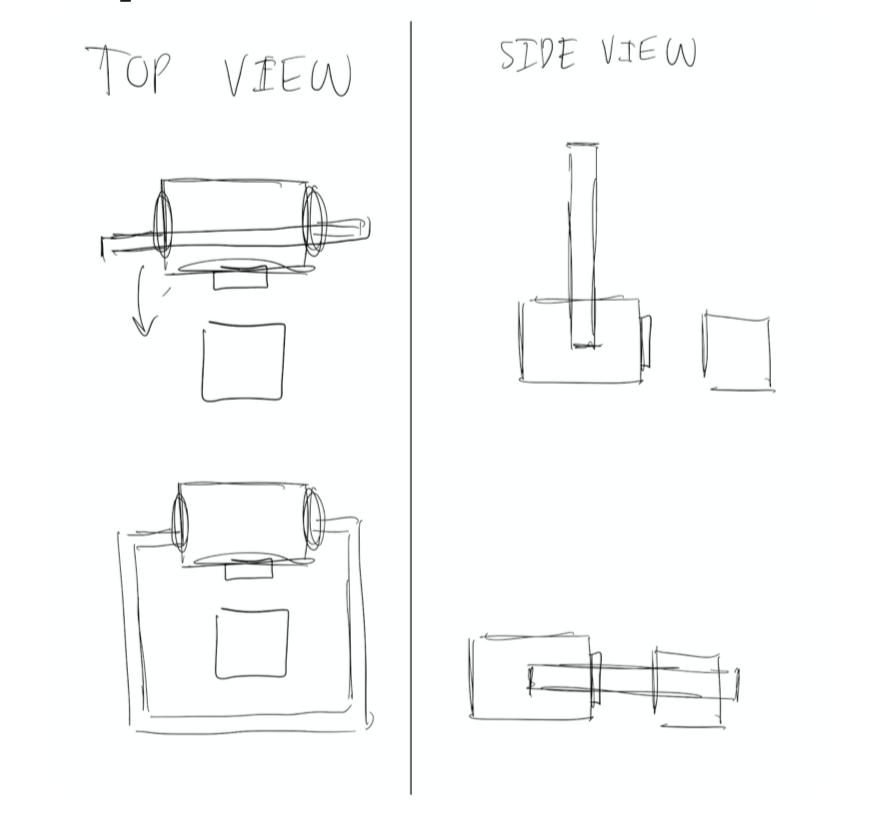
\includegraphics[width=8cm]{Design2}
    \caption{The Second Design}
\end{figure}


Based on the advantages and disadvantages of the first design we have come up with the second design. Instead of rotating around the vertical axis, the arms rotate around a horizontal axis, moving up and down . The advantage is that this design is still simple and symmetric. However, it suffers from the main fault that the sensor becomes useless once a block is collected. So it is not suitable for gathering multiple blocks.

\subsection{Preferred Design}


\begin{figure}[H]
    \centering
    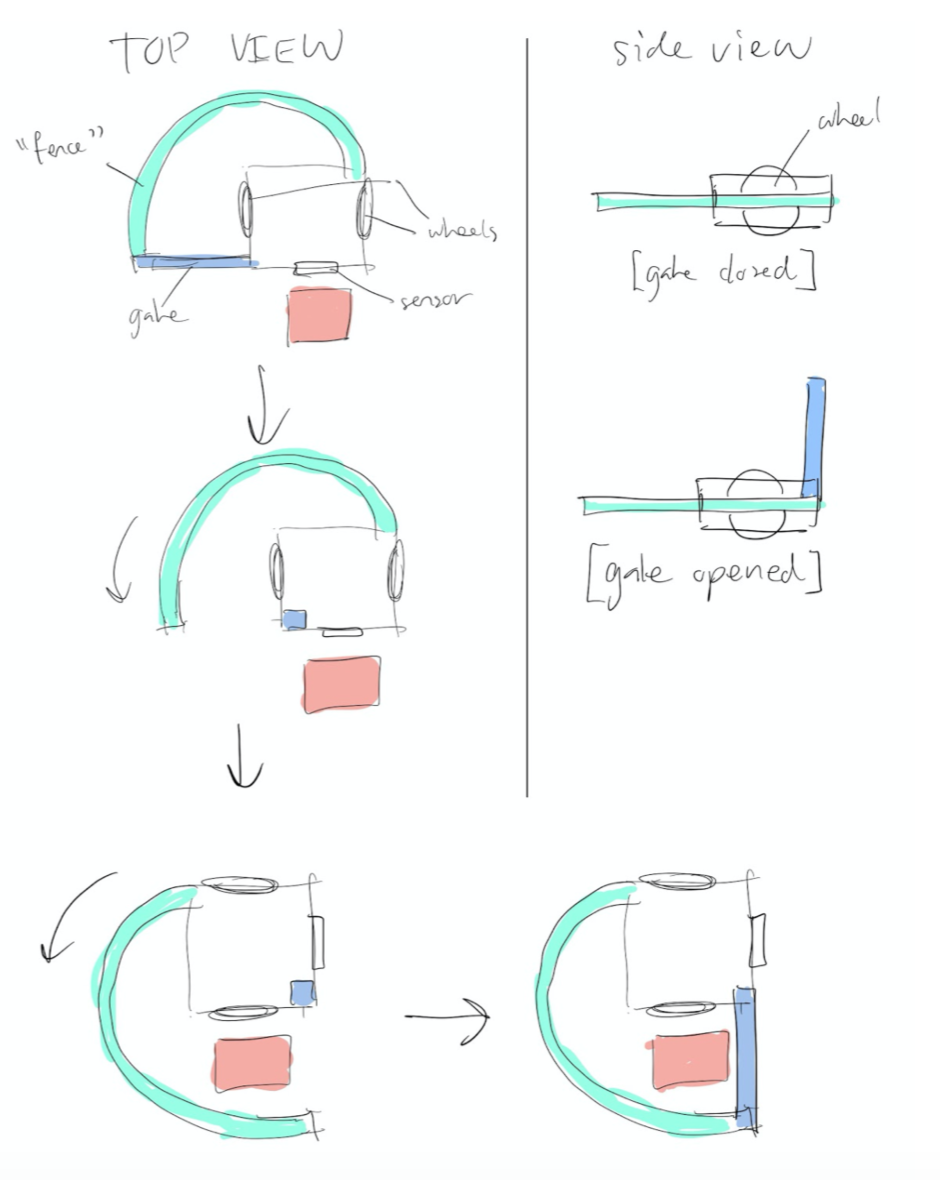
\includegraphics[width=8cm]{Design3}
    \caption{The Preferred Design}
\end{figure}


Here is our preferred design, which has a semi-circular arm that keeps the blocks in whilst collecting the blocks. This design is simple, suitable for collecting multiple blocks and it is easy to allocate sensors on the robot body. The circular shape also makes it easier to rotate. However, its asymmetric nature may make the robot prone to sway to one side. The robot also needs to rotate to collect to collect blocks which may increase complexity. Taking all this into account, we believe this design would be the best design as being able to collect multiple blocks could prove to be a huge advantage.









\section{Electrical}

The focus of the electrical team for the MVP has been to implement the sensors in Webots by looking up the properties from the datasheets. This is because it strongly informs the decisions of the software team and is hence on the critical path. A preliminary overview of the total parts can be seen in \cref{tab:parts_list}

\subsection{Sensor modelling}

The infra-red sensor is an analog signal, so it is susceptible to noise. This was modelled fairly conservatively with an estimate of $\pm50mV$ noise. This value was chosen partly to ensure robustness of the software to practical uncertainty, which is often higher than models suggest. Using this value along with the response characteristic in the datasheet, as seen in \cref{fig:ir_error}, the maximum range of the sensor is 1.2m. In Webots, distance sensors are modelled with Gaussian noise, $50mV$ was set to be three standard deviations. The field of view of the infra-red sensors was estimated from the datasheet to be 3$\deg$.

This signal can be measured accurately with the built-in arduino ADC, which has a resolution of $5mV$, an order of magnitude lower than our estimated noise.


\begin{figure}[H]
	\centering
	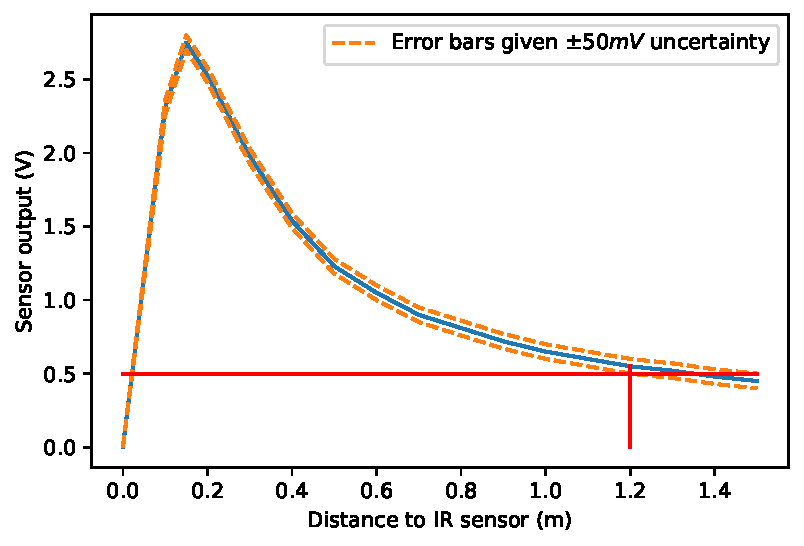
\includegraphics[width=0.6\linewidth]{ir_error}
	\caption{Estimate of the maximum range of the IR sensor}%
	\label{fig:ir_error}
\end{figure}

As the ultrasonic sensor requires precise timing, we must consider the characteristics of our microcontroller. The ATMega4809 supports input capture, which latches the value of the timer on an event such as a pin-state change. This allows an interrupt service routine to read the value of the timer more slowly, and still achieve near-clock-speed precision. Therefore there is no need to use discrete electronics for timing the ultrasonic pulse.

The distance error introduced per clock cycle is 20 $\mu$m (based on the speed of sound), whereas the resolution of the sensor specified on the datasheet is 3mm.  Therefore, we can be fairly confident that, with some care, the timing will not be a limiting factor. Adding a decent helping of random noise and so on, we have estimated here a maximum uncertainty of $\pm$5mm (taken in Webots to be three standard deviations). The field of view of the ultrasonic sensor was taken to be 30$\deg$ in accordance with the datasheet.

A summary of the distance sensors chosen can be seen in \cref{tab:distance_sensors}

\begin{table}[H]\centering
    \begin{tabulary}{\textwidth}{*{5}{C}}
    	\toprule
    	Sensor Type & Minimum Range (mm) & Maximum Range (mm) & Field of View & Error \\
    	\midrule
    	Ultrasonic & 20 & 1000 & 30\si{\degree} & \(\pm\) 5mm \\
    	IR (long) & 200 & 1500 & 3\si{\degree} & \(\pm\) 50mV \\
    	\bottomrule
    \end{tabulary}
    \caption{Comparison of chosen sensor types}
    \label{tab:distance_sensors}
\end{table}

The colour sensors will be implemented with 2 TEPT4400 light sensors, each covered with a red or blue filter to detect the respective colored light.  The signals are compared with threshold values (set by potentiometers) to establish colour of the LEDs. The comparison is done with discrete electronics so that it is simpler to tune the threshold value, and because the Arduino has only one ADC channel, which is used by the IR sensor.

The colour sensing will be simulated with two LightSensor nodes, with filters for each sensor detecting only red or blue light respectively. The proximity of the sensor necessary to detect the LEDs depends greatly on level of ambient light vs. LED luminosity, but 2.5cm distance from the LED is assumed to be sufficient in environments without excessive light pollution. The values sufficient in the simulation are to be confirmed.\\


\subsection{Initial electronics part list}

\begin{table}[H]\centering
{\renewcommand{\arraystretch}{1.5}
    \begin{tabulary}{\textwidth}{Lp{3cm}L}
        \toprule
        Item & Per-robot quantity & Notes \\
        \midrule
        Arduino Uno & 1 & \\
        Status LED & 6 & Controller state (3); Color sensor (2); Proximity
        sensor (1) \\
        Motor shield & 2 & \\
        Large motor & 2 & For the wheels \\
        Small motor & 1 & For moving the gate \\
        Ultrasonic sensor & 2 & \\
        Long IR sensor & 1 & \\
        Phototransistor & 2 & For color sensing \\
        Fixed resistor & requires further consideration & For converting the
        phototransistor characteristics to a voltage \\
        Dual comparator & 1 & For digitizing the color sensors \\
        Potentiometer & 2 & For trimming the color sensor
        threshold \\
        Fixed resistor & 2 & The other half of the comparator reference voltage
        divider \\
        Bypass capacior & requires further consideration & There will be
        significant motor noise to consider \\
        Main PCB & 1 & Contains status LEDs and any other required
        electronics \\
        Ultrasonic PCB & 2 & Adapts ultrasonic connector, as the default looks
        unreliable \\
        Color sensor PCB & 2 & Contains comparators and potentiometer voltage
        reference \\
        Arduino battery pack & 1 & \\
        Motor power supply & 1 & \\
        Misc connectors & requires further consideration & \\
        \bottomrule
    \end{tabulary}}
    \caption{Initial electronics part list}
    \label{tab:parts_list}
\end{table}


\subsection{System implementation}

The robots use the Arduino and its shield as the central communication hub. The sensor data is sent to the shield and then to the Arduino via PCBs, and the desired motor voltages are set by the Arduino, which powers the motors via the shield.


\begin{figure}[H]
    \centering
    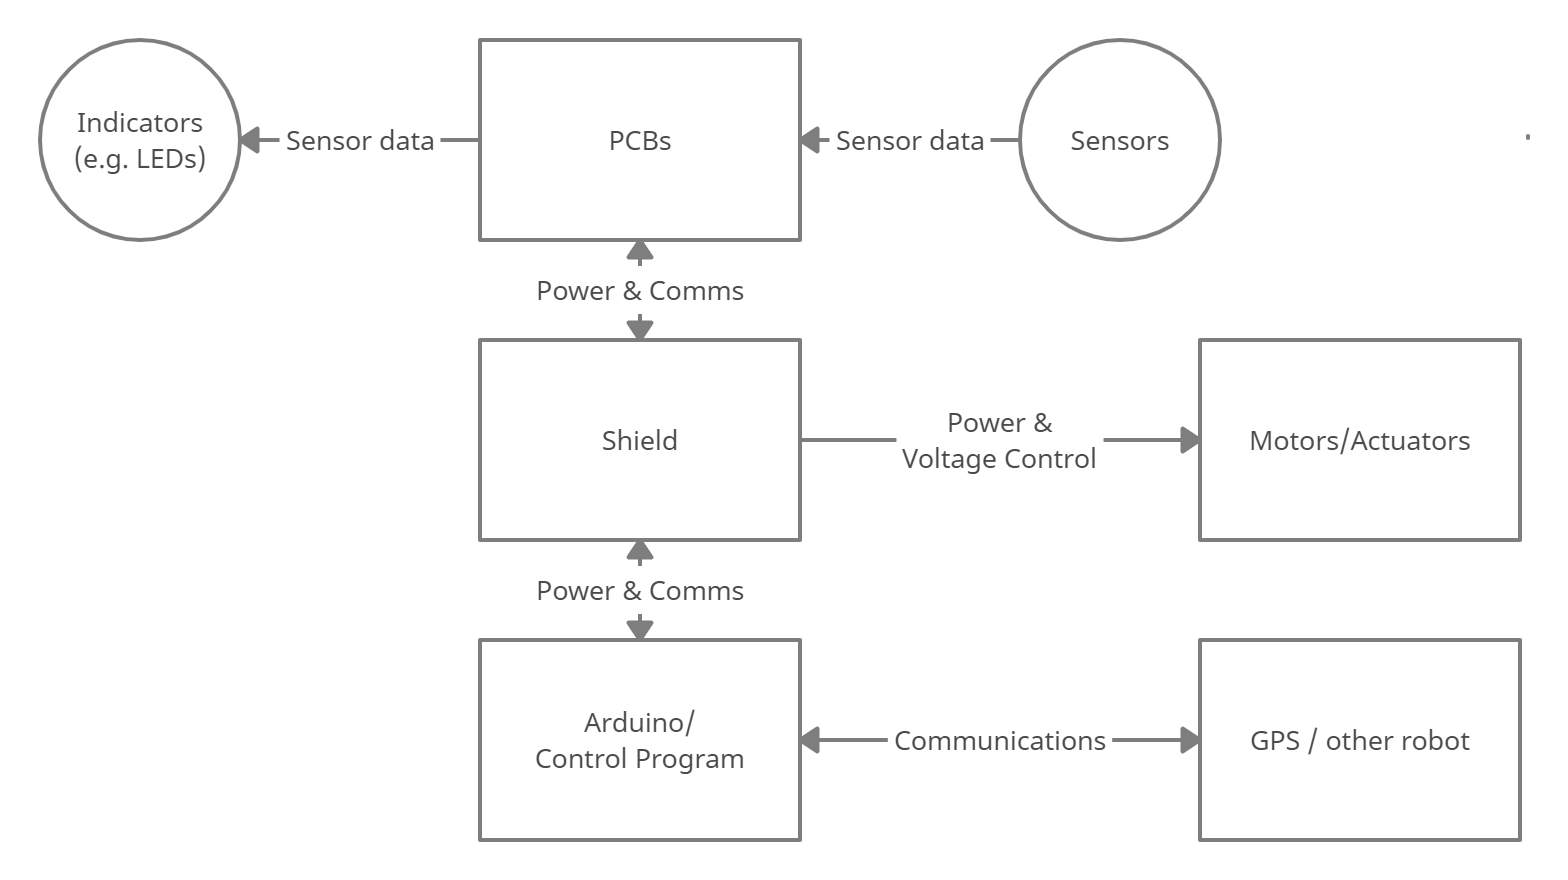
\includegraphics[width = 0.8\textwidth]{SystemDiagram.png}
    \caption{Overall System Diagram}
\end{figure}





\section{Strategy and Software}

The current software documentation (as of \today) can be found at \url{https://weixuanz.github.io/idp-v1/}.

\subsection{Overall Strategy}
\label{sec:software_flow_chart}

The main controller can be divided into four parts, the overall software flow chart is shown in \cref{fig:flow_overall}. The four parts are exploration and target selection algorithm, navigation and motion control, block collect control, and emergency interrupts.

We employed a coordinate system based approach (in the world frame), with heavy use of the GPS and compass data (OpenCV from the overhead camera). This approach, at a higher level, will allow more complicated strategies, as well as preventing collisions with the other robot and walls without any sensors. However, sensors are still used for interrupts, in additional to exploration and target selection.

There are two emergency interrupts, one to prevent collision, which uses input from the two ultrasonic sensor, faced at different angles to avoid avoid loss of signal when the incident angle is larger than 45\si{\degree}. This is because the long IR sensor has a minimum range of 20\si{cm}. The other interrupt exists as a backup strategy when the target coordinate is not exact, and the robot lose sight of the target when moving towards it. It will restart the target selection algorithm, trying to correct the course of the robot.

When the robot reaches the target, the block collect control program will check the colour of the block using data from the colour sensor to decide whether the block should be collected.

The target selection algorithm and navigation strategy are discussed in detail in \cref{subsec:target,subsec:motion}.

\newpage
\begin{figure}[H]
    \centering
    \includestandalone[width=0.8\textwidth]{./flowchart/overall}
    \caption{The overall software flowchart}
    \label{fig:flow_overall}
\end{figure}
\newpage

\subsection{Exploration and Target Selection}\label{subsec:target}

Whenever the robot needs a new target it rotates in a full 360º, scanning with its front-facing long IR sensor to detect objects. The IR sensor data generates peaks at close objects and using the distance data and robot bearing we can determine the position of the block in our co-ordinate system. If this object is a block this co-ordinate is passed to the motion controller. If the object is invalid, the other robot or a wall, then the next closest target is selected. When our robot gets close, if the block has the wrong colour then we choose the next closest target. This process is shown in a visual format in figures \ref{fig:flow_overall} and \ref{fig:flow_target}. Another possible algorithm is to use DBSCAN clustering on the coordinate-transformed coordinates.

Figure \ref{fig:sd_output} shows an example output of the IR sensor mapped onto the co-ordinates of the bots arena. The lines are rays from the sensor and the white circles are where it's hit an object or its maximum range.

\begin{figure}[H]
\begin{subfigure}[t]{0.5\textwidth}
    \centering
    \includestandalone[width=0.6\textwidth]{./flowchart/target_detect}
    \caption{The exploration algorithm}
    \label{fig:flow_target}
\end{subfigure}%
\begin{subfigure}[t]{0.5\textwidth}
    \centering
    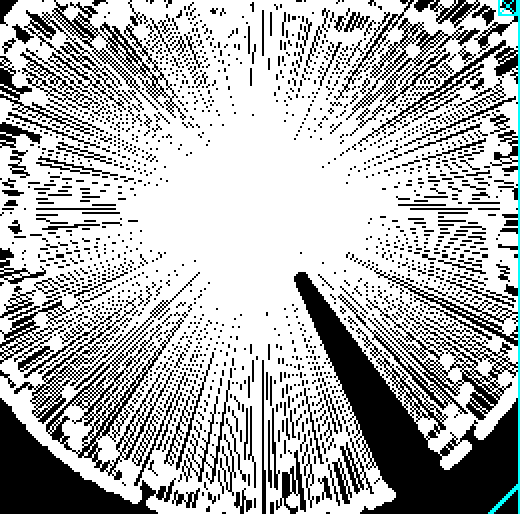
\includegraphics[width=0.6\textwidth]{sensor_output.png}
    \caption{Distant sensor output \footnotemark}
    \label{fig:sd_output}
\end{subfigure}
\caption{Exploration}
\label{fig:exploration}
\end{figure}

\footnotetext{Please note that the noise setting here was overestimated}

\subsection{Navigation and Motion Control}
\label{subsec:motion}

The robot moves according to a queue of target actions, involving target coordinates and rotations.

% this only works locally big rip
\begin{figure}[H]
    \centering
    \includestandalone[width=0.5\textwidth]{./flowchart/control_flow}
    \caption{Control logic for getting to a target}
    \label{fig:flow_motion}
\end{figure}

% I've included pretty much all the detail here so feel free to delete anything if needed, just make sure you understand first so you know what's deleted.

The motion control works by calculating wheel velocities based on the distance and the clockwise angle from the robot to target as illustrated in figure \ref{fig:flow_motion}. 3 parameterised methods are available for making this calculation. Each calculates a forward and rotational velocity, $V_f$ and $V_r$ respectively, which are combined to give velocities for each wheel motor. The left motor velocity is $V_f + V_r$ and the right motor is $V_f - V_r$. If the angle is negative the signs on $V_r$ are reversed. These outputs represent the fraction of the motors total drive. If any drive ends up over 1 it's capped at that value. For different actions i.e. rotate, drive to point etc. different methods can be used with different parameters.

The first method is purely angle based and is currently used for driving to positions. The velocities are given by the following equations where a and b are free parameters and x is the inputted angle. Currently a=3 and b=0.5.

\begin{equation}
    V_f =
    \begin{cases}
      0 & x\leq \frac{-\pi}{2} \\
      cos^a(x) & \frac{-\pi}{2} \leq x\leq \frac{\pi}{2} \\
      0 & \frac{\pi}{2} \leq x
   \end{cases}
\end{equation}

\begin{equation}
    V_r = (\frac{|x|}{\pi})^b
\end{equation}

The second method uses proportional control based on distance error for $V_f$ and angle error for $V_r$. Once combined into left and right velocities the result is passed through a sigmoid scaled to be from -1 to 1. In future this method will use full PID control. This method is currently used to face the robot at a particular bearing.

The third method uses a short linear region. In the equations below, a through d are parameters for the method and x and y are the distance and angle errors respectively. This method is used for rotating at constant rates with b and d being small.

\begin{equation}
    V_f =
    \begin{cases}
      -a & x\leq -b \\
      \frac{ax}{b} & -b \leq x\leq b \\
      a & b \leq x
   \end{cases}
\end{equation}

\begin{equation}
    V_r =
    \begin{cases}
      -c & y \leq -d \\
      \frac{cy}{d} & -d \leq y \leq d \\
      c & b \leq y
   \end{cases}
\end{equation}

% \subsection{Other Subsystems}

% \begin{figure}[H]
%     \centering
%     \includestandalone[width=0.3\textwidth]{./flowchart/collect}
%     \caption{todo}
%     \label{fig:flow_collect}
% \end{figure}



\subsection{Evaluation and Improvements}

% Other btec algo

Other algorithms and strategies were considered, for example, spiralling outwards from the starting point and collect blocks along the path. However, we think that the current strategy is more efficient, and have a higher potential while with similar feasibility. One of the main challenges of the spiral approach is keeping both robots on their spiral track without collisions, while keeping the strategy symmetric between the two robots running the same piece of control software.


% Potential failure

A robust target selection algorithm should be developed that overcomes all edge-cases. For example, it should limit the number of potential collisions. This can be achieved as the target coordinate will be checked against walls or the other robot when it is scanning for blocks. However, this does not guarantee that the paths of the two robots will not intersect after they start moving, so an emergency interrupt is crucial.

There is an extremely low probability that after the collision interrupt, the target choosing algorithm will pick the same target that triggered the interrupt, and the interrupt will be triggered again. In principle, this should not result in an infinite loop, since the main cause of an interrupt is the other robot, which should have moved after a few iterations.



In an unlikely situation, the distance sensors may not detect anything in the initial target selection phase. However, since the target selection algorithm will greedily choose the closest detected coordinate, which is guaranteed to exist (even if it is not an actual block but noise from the sensor), the algorithm will not stall.





A potential difficulty arises when the target block is of the wrong colour, which the target selection algorithm has to ignore. This can be partially solved by keeping a list of failed target coordinates as blacklisted regions. However, the block collector design would require the robot to drive backwards to prevent hitting the wrong block away from its current location.


Picking up the blocks may also be troublesome. Once the robot has detected and moved towards the block, it then needs to position itself correctly in order to pick up the block. How accurate this needs to be will need to be seen once we start testing our robot.


% we r currently planning to collect multiple blocks...
% The position of the areas themselves may cause trouble. Since the two areas are in the middle of the arena, they may disrupt the pathing of the robots if collected blocks there are collected blocks in the area. This may mean the robots would have to navigate their way around the area to prevent collisions or pushing blocks out of the area. Our current solution is to create a robot that will collect all the blocks at once, thus preventing this problem to occur at all.


% Improvements

A potential improvement to the current strategy after the MVP includes communication of coordinates of detected blocks of the wrong colour between robots, which will be inserted to the target priority queue with a higher profit. Furthermore, advanced probabilistic path planning can be implemented.

\subsection{Electrical Interface}

If the robot were to be physically made, an interface would be needed in order to test the software. This can be achieved by connecting LEDs in our circuits to act as feedback when a particular action is being executed. For example, an LED can be connected to the ultrasonic sensor such as to enable testing of the collision detection i.e. let the LED light up when an object is in front.

As the robot is implemented as a state machine (an inherited class from the Webots \texttt{controller.Robot}), another possible approach is to use an array of three LEDs to display a binary number, indicating the current state of the robot (e.g. target selection, moving to target, etc).

\end{document}
